\section{Results}\label{sec:results}

\subsection{Mechanism Combinations}\label{subsec:mechanism-combinations}
The absolute mean error as a percent of the total preference space by coordination
mechanism per voting mechanism is graphed in
\autoref{fig:vm-col-cm-hue-error-as-percent-of-space-abs-mean}.
% 04/13: \vicki{Briefly describe how you define mean square error}
The absolute mean error as a percent of the total preference space
$\sigma_{\lvert M\% \rvert}$  is defined as
$
    \sigma_{\lvert M\% \rvert} =
    \frac{1}{n (\systemspace_{\max} - \systemspace_{\min})}
        \sum^{n}_{i = 1}{\lvert \epsilon_i  \rvert}
$,
where $n$ is the number of runs, $\systemspace_{\max}$ and $\systemspace_{\min}$ are
the maximum and minimum value in the preference space, respectively, and $\epsilon_i$
is the error of run $i$.
Error is defined as $\truthof{\text{proxy}}~-~\truthof{\text{baseline}}$, meaning the
output of the proxy run minus the output of the baseline (all agents voting).

From this plot, there are a few trends that are immediately identifiable.
First, error unsurprisingly increases as the number of inactive agents increases.
This is true with two notable exceptions: first, the Active Only/Median
mechanism combination has a somewhat sawtooth shape.
This is due to the Median mechanisms always choosing a specific agent's preference
instead of aggregating to some more preferential in-between value.

The second exception is that Mean coordination mechanism consistently dips when all but
one agent become delegators.
This is because we take the mean of the constituents and the proxy, then apply the
voting mechanism on the set of proxy-constituent votes.
Since there is only one agent, there is only one proxy-constituent vote and so the
result of the vote is the result of the coordination mechanism.
Essentially, the coordination mechanism replaces the voting mechanism.

We can also see the Mean and Median coordination mechanisms generally yield similar
amounts of error.
In particular, when either of these mechanisms is combined with the Mean voting
mechanism the results are very similar to when all agents are active and able to vote.

Notably, the Expert coordination mechanism works worse than the others as the number
of delegators reaches a significant portion of the population.
In particular, the Expert mechanism tracks nearly identically to Active Only when
using the Midrange voting mechanism.
Depending on the use case, this may or may not be beneficial.
If we are attempting to find the best result for all agents, this mechanism may yield
undesirable results.
However, if we are attempting to exploit the expert's experience, as described
by~\cite{Miller1969}, this error could actually be considered an improvement over
the original result.
This is because the experts were able to influence and change the vote, presumably
bringing it closer to what their expertise dictates.
Nevertheless, when the number of delegators is low, the Expert mechanism works
similarly to the other coordination mechanisms.

Importantly, it is clear that using proxy voting, regardless of the mechanisms used,
is better than losing information by not allowing inactive agents to vote in any way.

\subsection{Inactive Penalty}\label{subsec:inactive-penalty}
What if we were to introduce some penalty for the inactive agents?
Since they aren't participating as much, perhaps it would be fair that their voice is
not as strong.
We attempted the same experiments as above with different weights between a proxy and
their constituents.
Specifically, the proxies maintain their weight of 1, while their constituents have
their weight reduced to $\sfrac{1}{5}$ (0.2) of their original weight.
We choose $\sfrac{1}{5}$ because it still allows constituents to have some impact
while still having their influence significantly reduced.
The difference between all agents voting and proxy voting of such a setup are
shown in~\autoref{fig:different-weight-comparison}.
% 04/13:
% \vicki{
%     How do you define error in this case?
%     If you only give them a .2 vote, but compare to when they get a full vote, that
%     seems meaningless.
%     We are giving them a .2 vote because their vote shouldn't count as much.
%     Can you compare the shift in results between the two methods?
%     I wouldn't call it an error, but the difference between the methods.
%     Better to have the comparison between the two on one graph rather than
%     having the reader compare two figures.
% }

\begin{landscape}
    \begin{figure}[p]
        \centering
        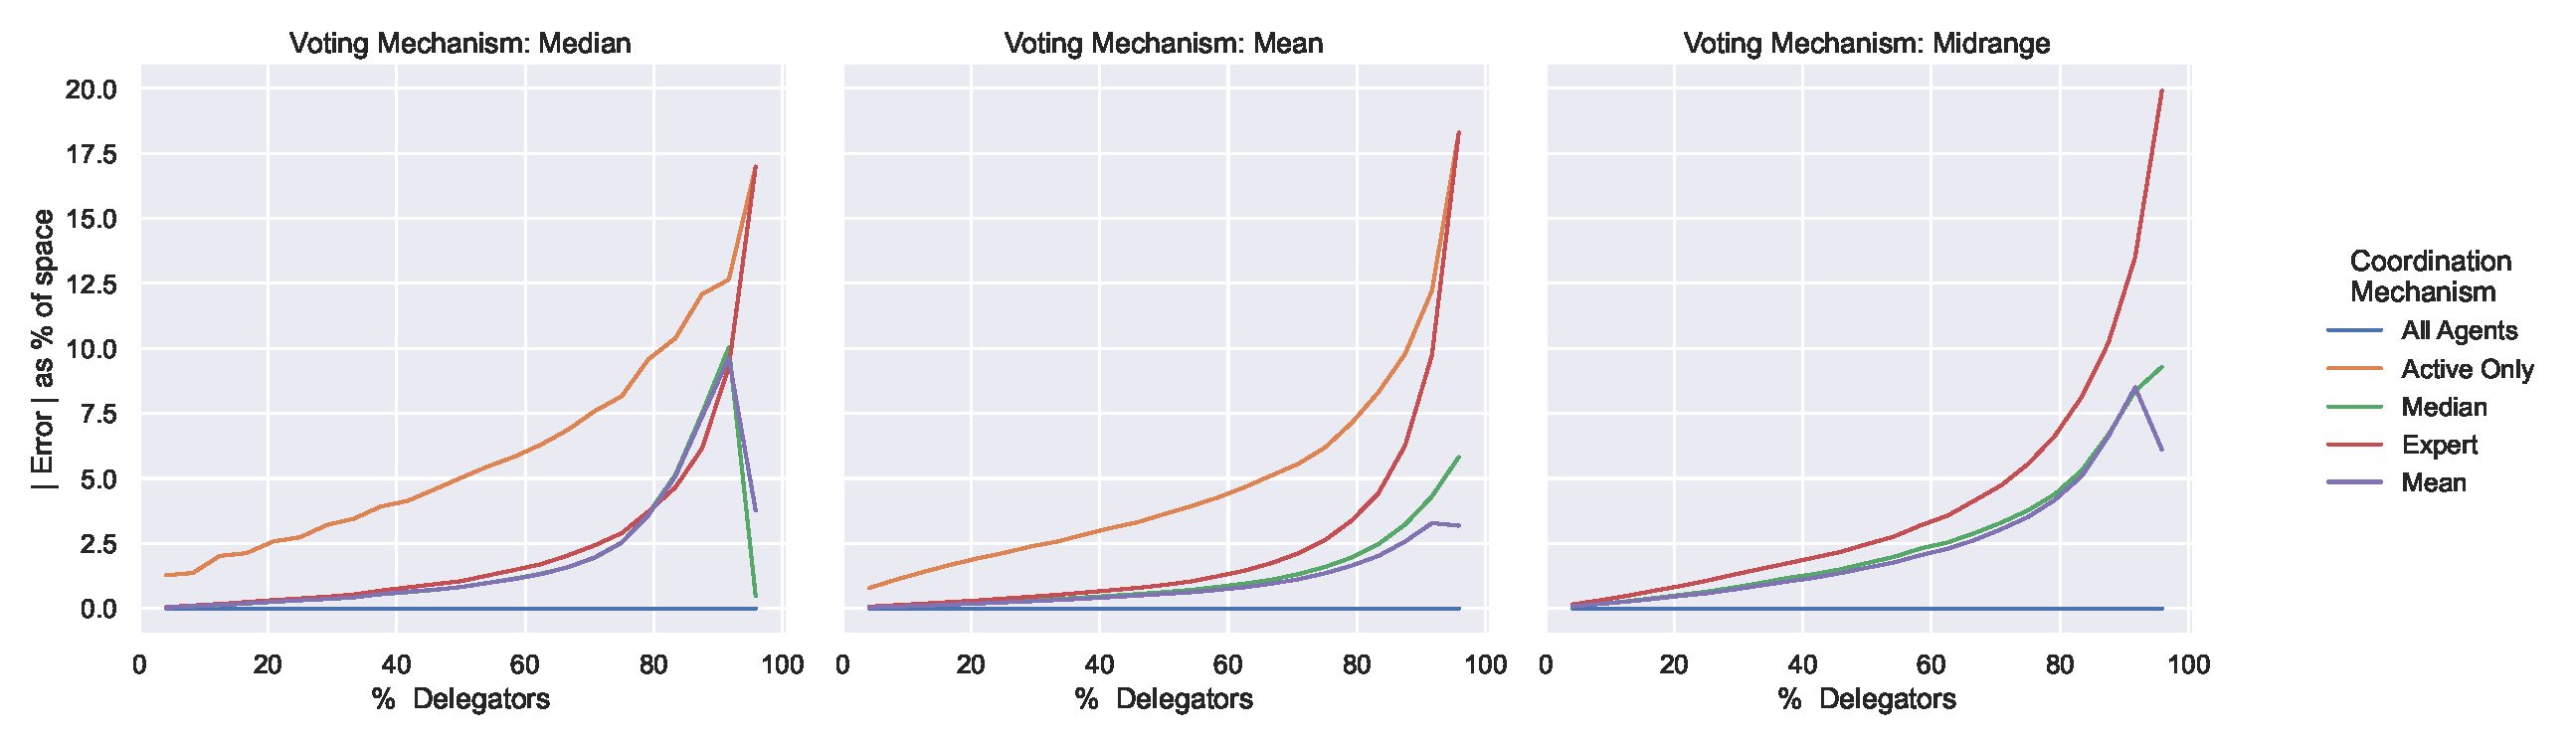
\includegraphics[scale=0.55]
        {content/chapter2/figures/vm_col_cm_hue_error_as_percent_of_space_abs_mean}
        \caption{
            The absolute mean error as a percent of the preference space by
            coordination mechanism per voting mechanism.
            `Error as a percent of the preference space' means the error divided by
            the total size of the preference space.
            Note All Agents represents when all agents are voting, meaning no proxy
            voting is used and all agents are present.
            Similarly, Active Only represents when proxy voting is not used and not
            all agents are present, and when proxies lose their constituents.
            The results are averaged over 1024 total runs.
            There are 24 total agents.
        }
        \label{fig:vm-col-cm-hue-error-as-percent-of-space-abs-mean}
    \end{figure}
\end{landscape}

\autoref{fig:different-weight-comparison}~shows there is an immediate difference from
when all agents have the same weight.
This is because, due to the weight, there is a shift towards the proxies' preferences
instead of the inactive voters'.
% 04/13: \vicki{which graphs are you referring to?  due to what?  unclear.}
% MDH: The referred-to graphs are specified in the previous sentence.
% I've re-referenced it here for clarification.
% The explanation for the error is in the next sentence.
Depending on the situation, this may be desirable.
Since the inactive agents are not participating they may not have as much information
and so their preference may not be as `up-to-date' as those who are actively
participating.
In situations where new information is constantly being introduced, such penalties
could be very valuable to ensure the most current information is being used.

Notably, the Median voting mechanism suddenly takes a sharp dip and produces a result
closer to all agents voting with the difference in weight.
This is strange since it is completely different compared to how any other
combination, or even the same combinations with less inactive voters, works.
With some inspection, one can find this dip is due to active voters having a
significantly larger influence compared to inactive voters.
With this setup, an active voter is worth 5 times the amount of weight than an
inactive voter.
Therefore, when an active voter's weight is added to the sum it is more able to push
the sum over the half-way mark, thereby making that active voter's preference the
median.
This is also why we see the most extreme dip with using the Median voting mechanism
with Median coordination mechanism: the proxy is able to reach the median both when
coordinating and when voting, thereby making the proxy and its constituents' vote be the
proxy's preference.
This makes the system less volatile, since votes are less likely to be an inactive
voter's, and so we don't see the large spike in error when a large percent of agents
are delegating.

Additionally, from~\autoref{fig:different-weight-comparison}, we see both the Median
and Mean voting mechanisms quickly increase
% 4/26/2023: \vicki{quickly increase in error? explain.  This is interesting as more
% delegators slows the affect. Better if x axis goes to 100\% as the other tables do.}
in difference before beginning to level out.
This is again due to the difference in weight between the active and inactive voters.
When both types of voters have the same weight, the coordination mechanisms help
ensure the loss of preference from the agent going inactive is minimal.
However, when they have different weights, in particular when the weight of the
inactive voters is substantially less than that of the actives, the results are more
akin to when the voter doesn't vote.

The Midrange voting mechanism, however, does not increase as quickly and does not
achieve as much of a difference.
Midrange, or $L_{\infty}$, takes the highest and lowest voting and averages the two.
This means it ignores weight, which is likely why the change in weights does not
affect it as much.
Any difference in the outcome, then, must come from the coordination mechanisms used
prior to the final vote being calculated with Midrange.

Notably, the Median mechanisms, both voting and coordination, yields the largest
change.
Mean is close behind, and Expert yields slightly less.
Since the Median voting mechanism has already been shown to be difficult to
manipulate~\cite{Moulin1980}, using both a Median voting and Median coordination
mechanism would likely be a good choice when choosing which mechanisms to use.

\begin{landscape}
    \begin{figure}[p]
        \centering
        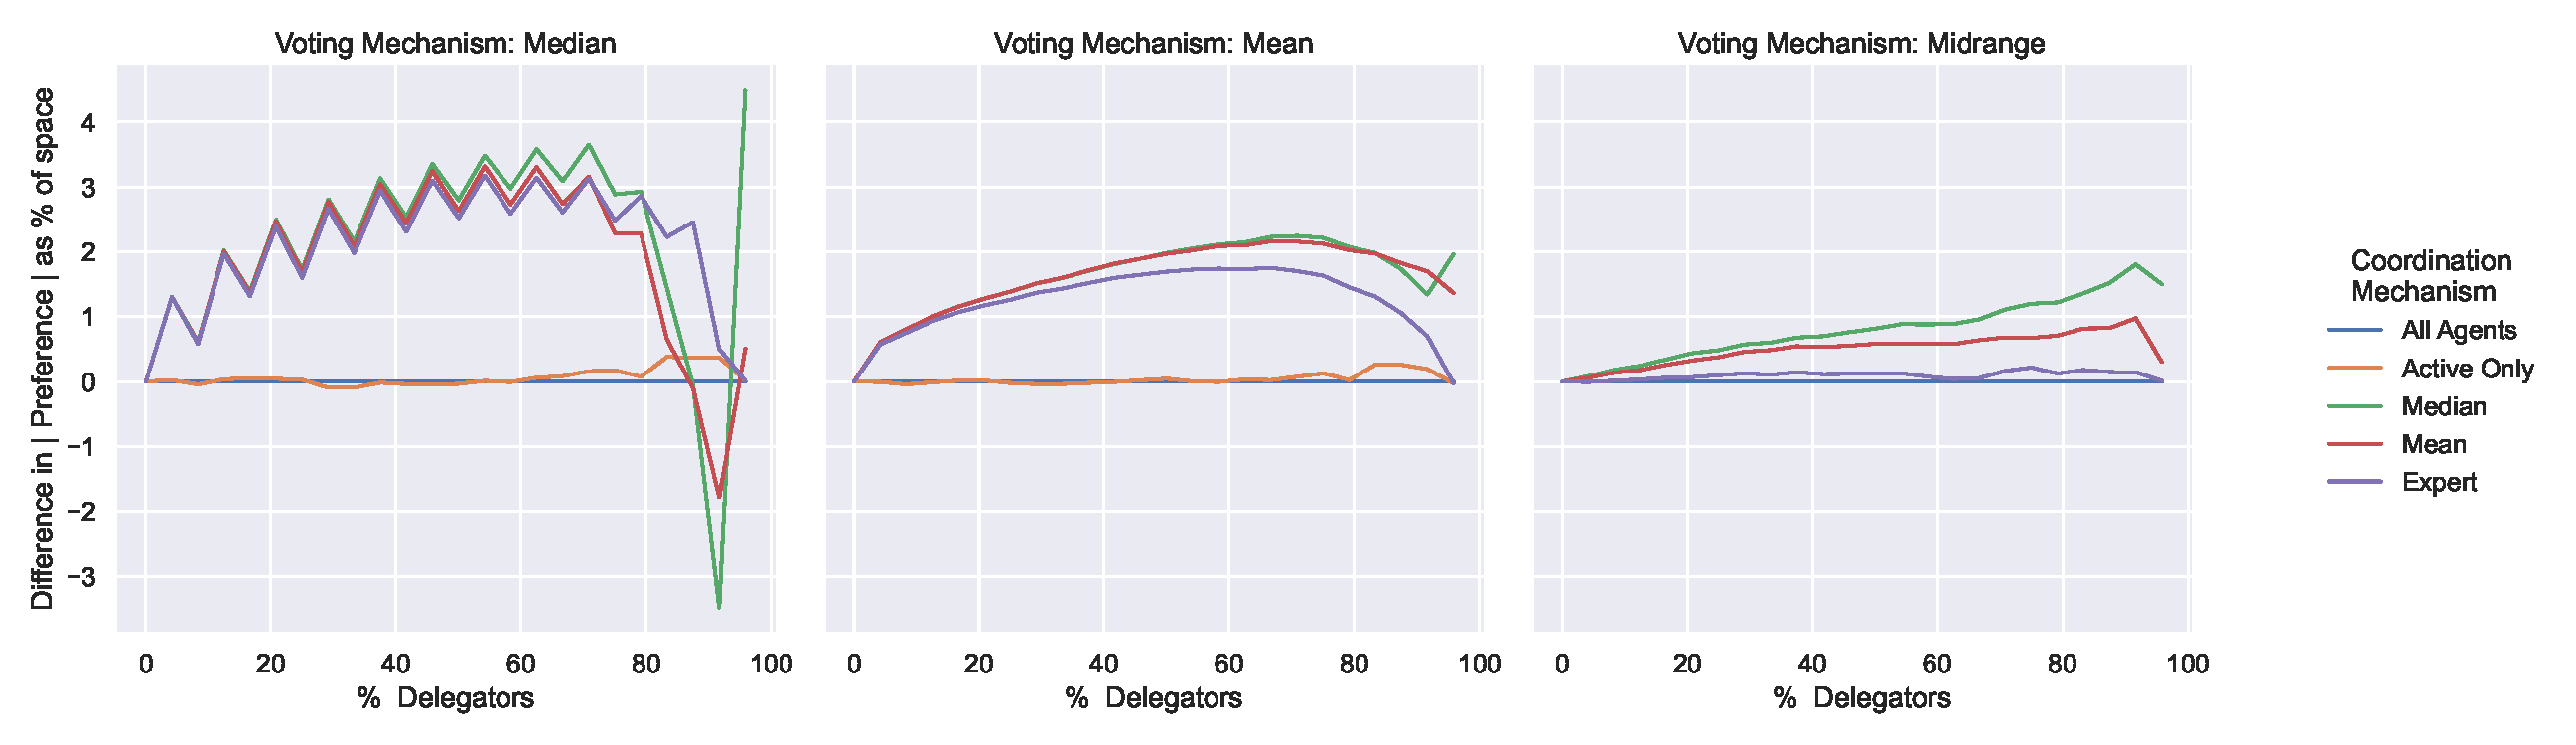
\includegraphics[scale=0.55]
        {content/chapter2/figures/different_weight/difference_abs_pref_percent_of_space}
        \caption{
            The difference between all agents having the same weight and inactive
            agents having only $\sfrac{1}{5}$ the weight as their proxies.
            The difference is in terms of distance as a percent of the preference
            space from all agents voting.
            `Distance as a percent of the preference space' means the absolute
            difference divided by the total size of the preference space.
            The results are averaged over 1024 total runs.
            There are 24 total agents.
        }
        \label{fig:different-weight-comparison}
    \end{figure}
\end{landscape}

\subsection{By Distribution}\label{subsec:results-distribution}
\autoref{fig:distribution-error-as-percent-of-space-abs-mean} shows
the absolute error as a percent of the preference space by coordination mechanism for
each voting mechanism and preference distribution.
\autoref{fig:distribution-different-scale-error-as-percent-of-space-abs-mean} shows
the same graphs, but with a different scale for each plot to more easily see the shape.
Additionally, each graph is zoomed in for readability
in~\autoref{apx:error-by-dist-zoomed}.

\begin{figure}[p]
    \centering
    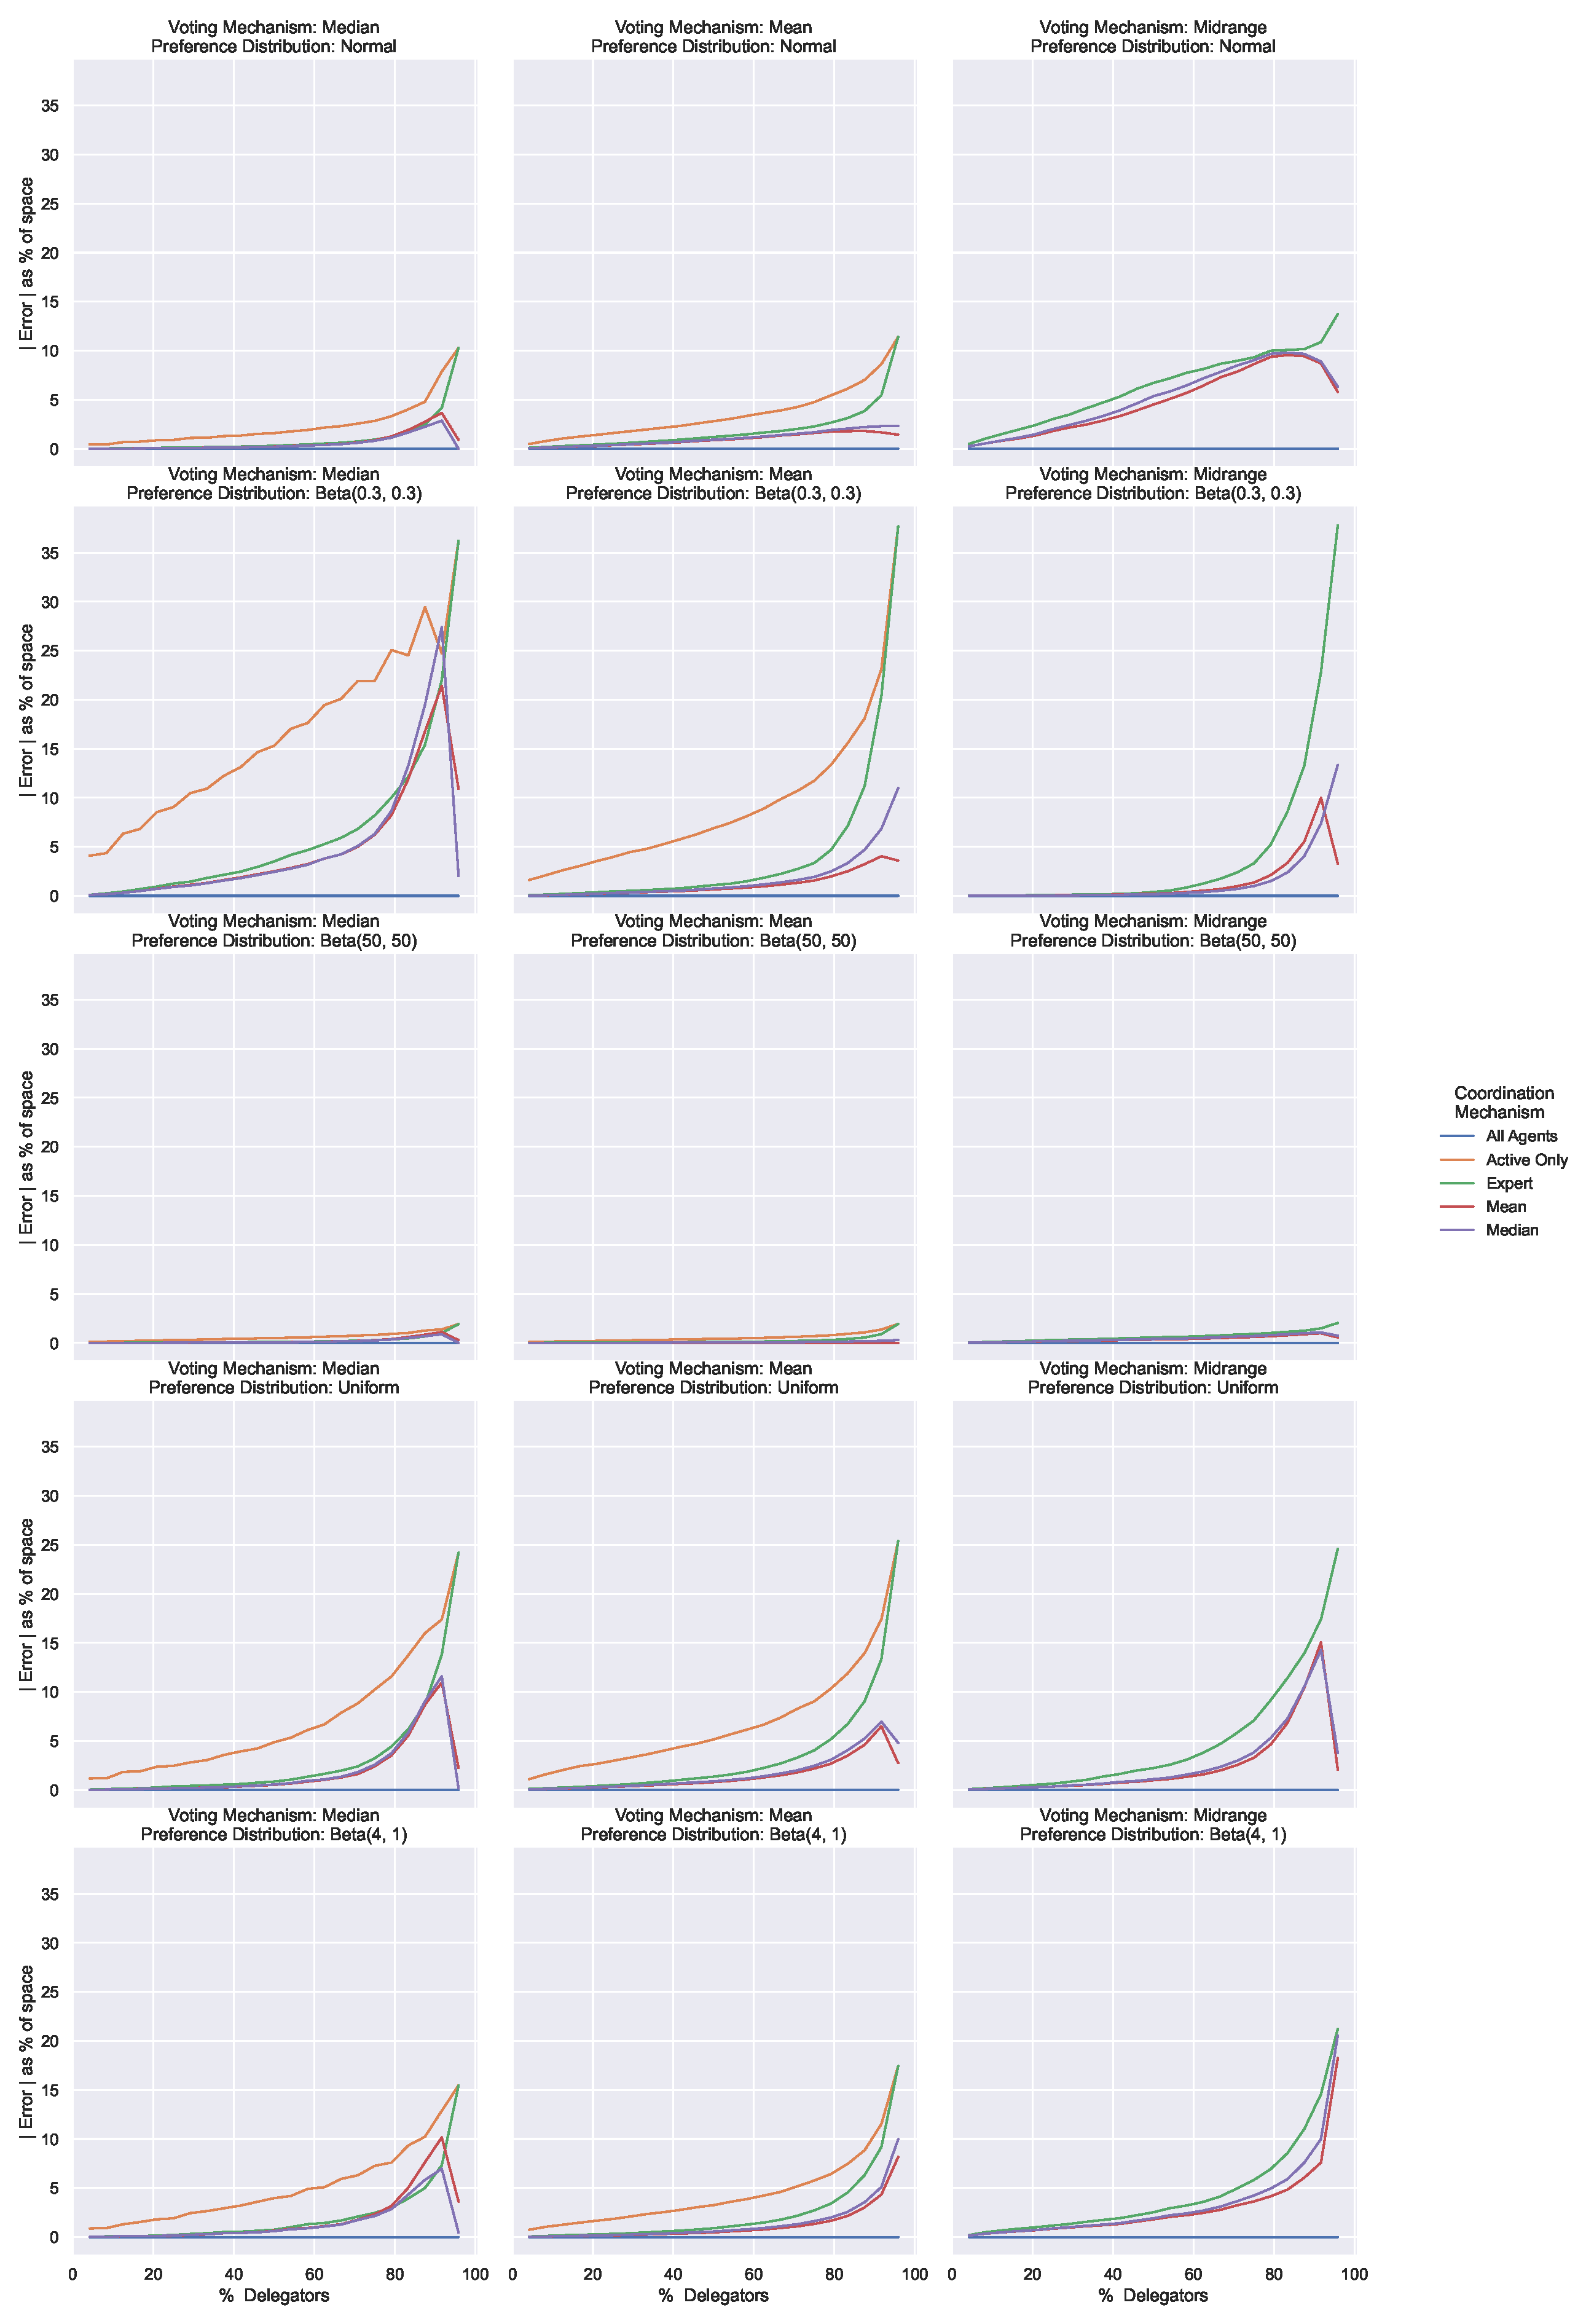
\includegraphics[scale=0.35]
    {content/chapter2/figures/distribution_error_as_percent_of_space_abs_mean}
    \caption{
        The absolute error as a percent of the preference space by coordination
        mechanism for each voting mechanism and preference distribution.
        The results are averaged over 1024 total runs.
        There are 24 total agents.
    }
    \label{fig:distribution-error-as-percent-of-space-abs-mean}
\end{figure}

Unsurprisingly, the tighter the probability density function (PDF) of a distribution,
the less error it has overall due to many votes being close to each other.
\betadistribution{50}{50} and Normal are two such distributions.
Nevertheless, these plots show the increase in error is consistent regardless of the
mechanisms or distributions used.
Mean and Median coordination mechanisms show a similar amount of error, while Expert
shows slightly more except when a large portion of the population is delegating and
when using the Midrange voting mechanism.
Interestingly, this seems to indicate again that it does not matter how you do proxy
voting so long as it is done.
Additionally, it should be noted the mechanisms perform well on most preference
distributions, including the asymmetrical distribution \betadistribution{4}{1}.

Unfortunately, while the error for other distributions is relatively similar,
\betadistribution{0.3}{0.3} yields considerably more error and starts accumulating
this error earlier when using the median voting mechanism.
\betadistribution{0.3}{0.3} represents a highly polarized topic, with its probability
density function having large spikes at either end of the preference space, making it
extremely important to ensure results are fair and accurate.
This would indicate that proxy voting, while it is still better than active-only
voting, does not work quite as well when agents have stronger, opposing opinions.
% 04/13:
% \vicki{
%     Why does this happen?
%     Is it because there are so few voters?
%     It would seem that two strong opinions shouldn't cause more error.
%     This needs to be explored as two opposing opinions is a common case.
% }
% MDH: See the following paragraphs where I explain why this could be.
% I've made a slight edit to specify this error really only occurs with the median
% voting mechanism.

For the median mechanism voting mechanism, the increase in error makes sense.
The median will most often be the preference of a specific agent, instead of some
value in between.
As such, the result will often be in one of the spikes in the PDF, since that is
where the majority of the agents' preferences will be, yielding higher error than when
using the Mean or Midrange voting mechanisms.
With the other voting mechanisms, the error is similar to other distributions using
the same mechanisms until the vast majority of the agents are inactive.
The increase in error is because as more agents go inactive there are fewer agents able
to serve as proxies, and so there may not be as desirable of a proxy to represent
each agent.

This finding is particularly important, as often the most polarizing topics are the
most important to individuals.
While it is still more beneficial to use proxy voting than not, in these polarized
cases, agents should make an extra effort to participate in-person to learn all they
can about the topic and ensure their voice is heard.
Those using proxy voting on split issues ought to be aware of this weakness and
implement some limitation to prevent inaccurate results.
These limitations could include requiring some percentage of the population, say
20--30\%, to be active.
Alternatively, if it becomes apparent that discussion is changing the opinions of the
active voters, which could be learned by occasionally polling the participants, it
may be wise to require voters to attend in person.
That way, those who have not been present to attend the deliberations can properly
participate.

\subsection{Preference Change}\label{subsec:results-shift}
\autoref{fig:abs-diff-from-preference-change-error-as-percent-of-space-abs-mean} shows
the difference in error between when proxies do have a preference change and when
they don't.
In this case, the proxies were able to shift their preferences by up to 10\% of the
total preference space, while delegators kept their original preference.
This represents the proxies changing their preference for an issue after deliberation.

Unsurprisingly, the amount of error increases as more agents become inactive.
However, the coordination mechanisms are much more tightly grouped than in other
scenarios.
We also see all voting mechanisms actually yield worse error than active-only
voting when using the Median and Mean coordination mechanisms.
This might be because delegators are selecting proxies who then shift a large amount,
leaving the delegator unsatisfied.

This potentially worse outcome highlights not only the importance of actively
participating in discussions, but also that when one needs to choose a proxy the
proxy must be someone who would act as the delegator who want them to act.

\begin{landscape}
    \begin{figure}[p]
        \centering
        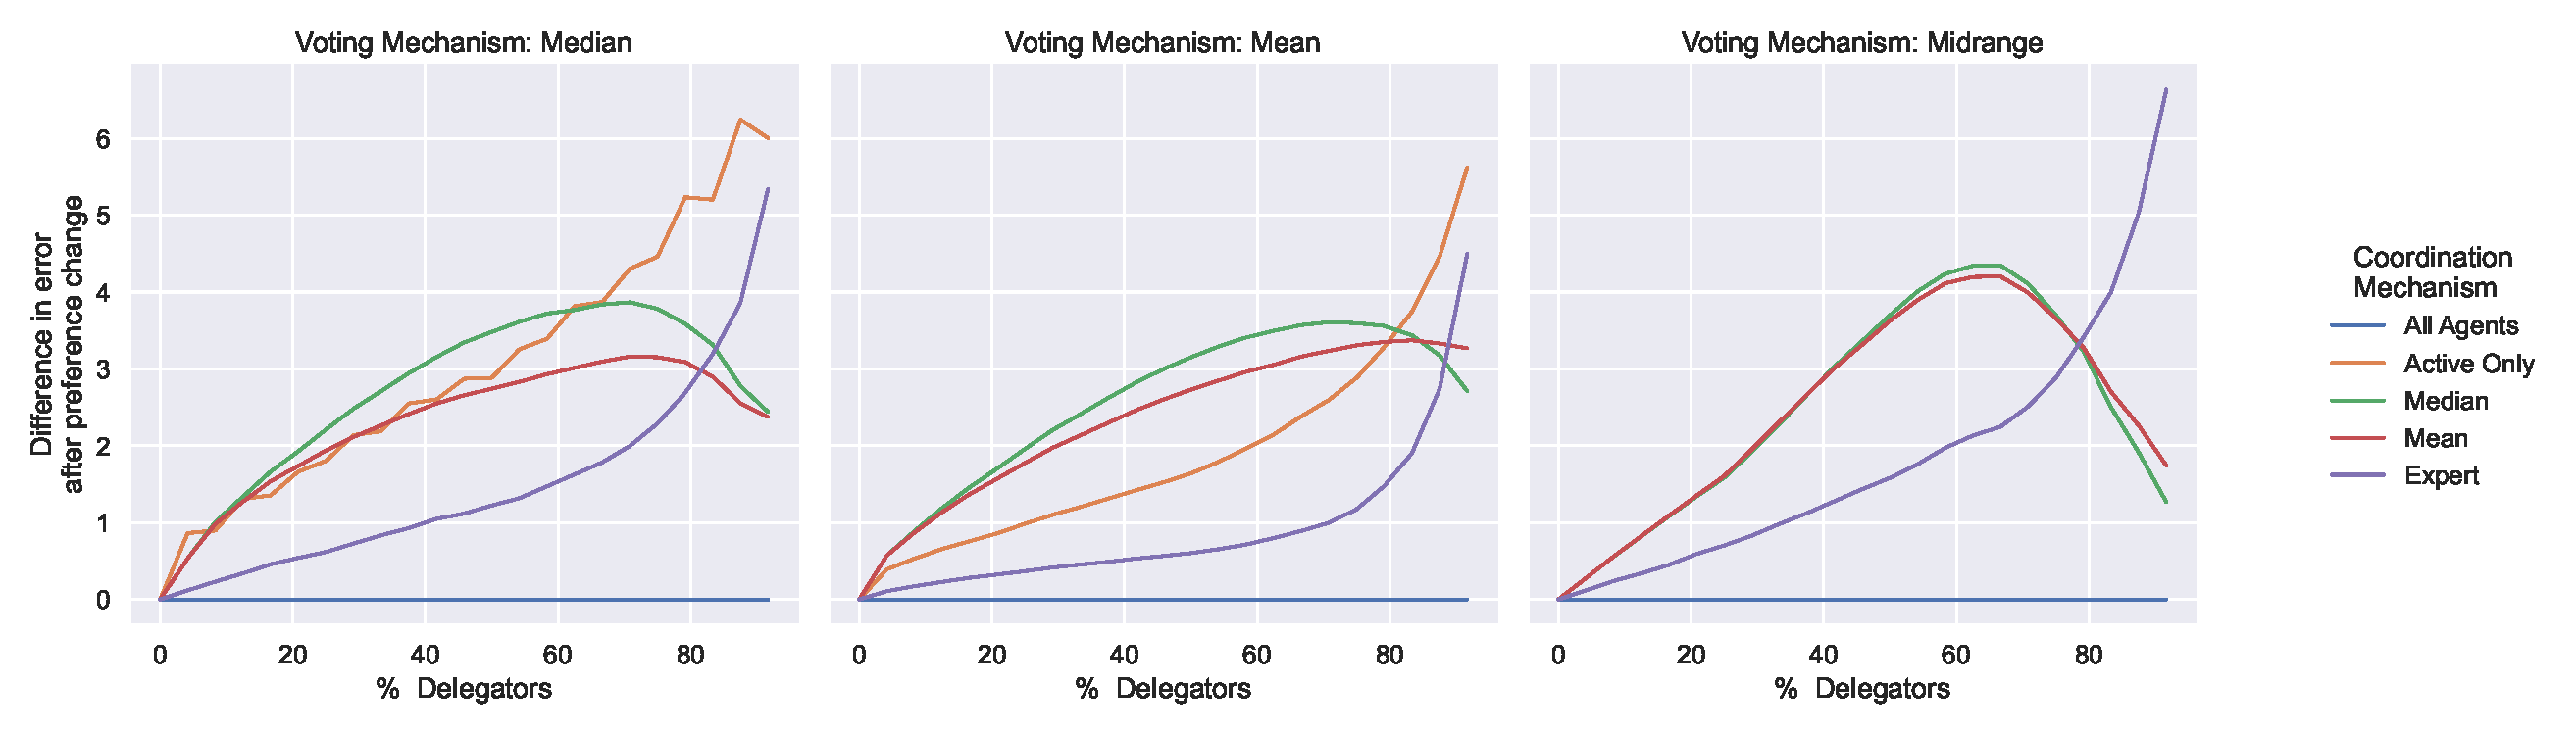
\includegraphics[scale=0.55]
        {content/chapter2/figures/abs_diff_from_preference_change_error_as_percent_of_space_abs_mean}
        \caption{
            The absolute difference in the error produced between without a
            preference change and with a preference change as a percent of space.
            The results are averaged over 1024 total runs.
            There are 24 total agents.
        }
        \label{fig:abs-diff-from-preference-change-error-as-percent-of-space-abs-mean}
    \end{figure}
\end{landscape}
